\section{Adaptation gains across evaluated pairs}
\label{sec:heterogeneity}
The pair-level curves reveal how broadly the aggregate gain extends. Figure~\ref{fig:pairs} gives each pair the same axes and retains the anonymous identifiers supplied by the scorer. Every pair finishes below its own zero-label Brier error. The magnitude varies substantially: pair ALC ranges from 0.068828 to 0.246809. Six pairs have at least one intermediate increase, accounting for eight of the 45 adjacent transitions, while the final-budget gain is shared by all nine.

\begin{figure}[H]
\centering
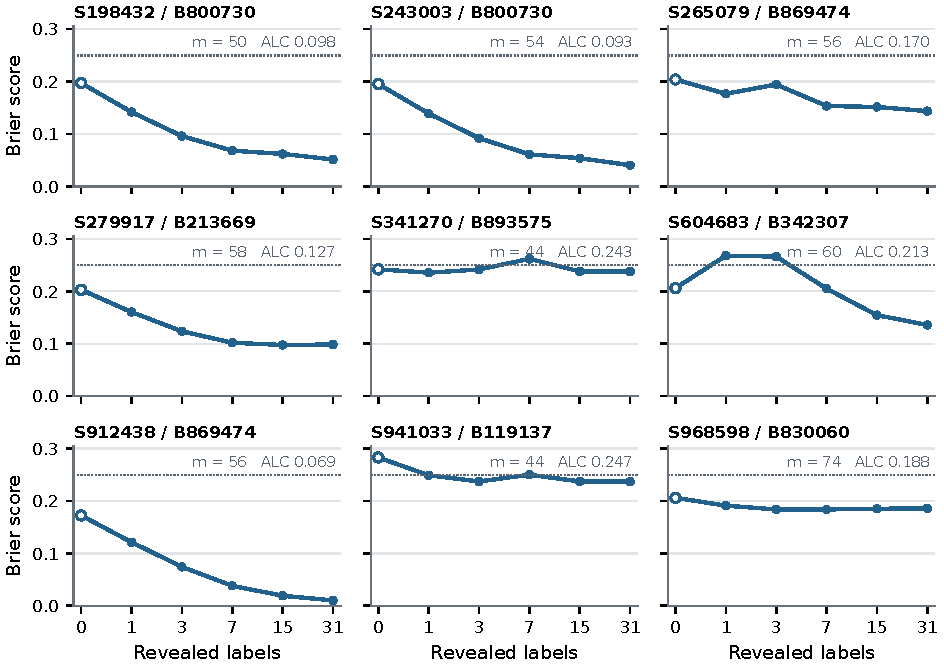
\includegraphics[width=.98\linewidth]{figures/pair_learning_curves.pdf}
\caption{All nine pair learning curves, with a common Brier scale. S and B abbreviate the published anonymous subject and benchmark prefixes; $m$ is the number of distinct evaluated subject--item pairs. Open markers show the initial forecast. Dotted lines show the fixed-0.5 reference. The horizontal positions use the same logarithmic budget transformation as Figure~\ref{fig:macro}.}
\label{fig:pairs}
\end{figure}

\begin{table}[H]
\centering
\caption{Pair-level results. Gain is $B_0-B_{31}$; larger values indicate more improvement.}
\label{tab:pairs}
\small
\begin{tabular}{@{}llrrrr@{}}
\toprule
Subject & Benchmark & $m$ & ALC & $B_{31}$ & Gain \\
\midrule
198432 & 800730 & 50 & 0.098321 & 0.051231 & 0.145805 \\
243003 & 800730 & 54 & 0.092645 & 0.040327 & 0.154904 \\
265079 & 869474 & 56 & 0.169868 & 0.143456 & 0.060445 \\
279917 & 213669 & 58 & 0.126733 & 0.098363 & 0.104464 \\
341270 & 893575 & 44 & 0.243301 & 0.237775 & 0.004090 \\
604683 & 342307 & 60 & 0.212877 & 0.135660 & 0.070355 \\
912438 & 869474 & 56 & 0.068828 & 0.010232 & 0.162210 \\
941033 & 119137 & 44 & 0.246809 & 0.237130 & 0.045958 \\
968598 & 830060 & 74 & 0.188016 & 0.185867 & 0.020278 \\
\bottomrule
\end{tabular}
\end{table}

\paragraph{Three useful patterns.}
S912438 shows how strongly a small support set can sharpen a forecast: its Brier error falls from 0.172442 to 0.010232, a 94.07\% reduction. S604683 illustrates recovery as evidence accumulates: error rises to 0.267988 after one label, then falls to 0.135660 by the final budget. S341270 has a modest gain of 0.004090, identifying a setting where richer item structure could be valuable. Together, these trajectories suggest a practical development strategy: preserve rapid adaptation where it succeeds and target additional modeling capacity at the flatter curves.
